\documentclass{thesis}

% Meta-data
\title{基于STM32的物联网智能导盲杖设计与仿真实现}
\author{张三}            % 需用户自行修改
\studentID{2022xxxx}    % 需用户自行修改
\theclass{电子信息工程22xx}    % 需用户自行修改
\advisor{李四}          % 需用户自行修改
\college{信息工程学院}   % 需用户自行修改
\date{2026年5月}

\usepackage{tikz}
\usepackage{lipsum} % For generating placeholder text to demonstrate volume if needed, but I will write real text.
\usetikzlibrary{shapes,arrows,positioning,fit,calc,automata}

\begin{document}

% Create Cover
\makecover

% Abstract
\begin{cnabstract}
    据世界卫生组织统计,全球视力受损人数众多,视障人士在独立出行时面临着严重的导航与安全挑战。传统的盲杖仅能探测地面障碍物,无法检测头部或腰部高度的悬空障碍,且缺乏定位与求助功能。随着物联网(IoT)技术与嵌入式系统的飞速发展,将智能化技术引入辅助器具设计,开发一款集环境感知、实时报警、远程监控于一体的智能导盲杖,对于提升视障群体的生活质量和社会融入度具有重要意义。

    本文设计并仿真实现了一款基于STM32微控制器的物联网智能导盲杖系统。系统以STM32F103C8T6为核心控制单元,集成了HC-SR04超声波测距模块、OLED显示模块、蜂鸣器报警模块及按键输入模块。在设计方案中,创新性地引入了“物联网模拟仿真”的概念,利用Proteus仿真软件构建系统电路,并通过OLED屏幕模拟WIFI模块的数据传输状态,实现了对智能硬件联网功能的验证。

    系统主要功能包括:(1) 多维障碍物检测:利用超声波传感器实时探测前方障碍物距离;(2) 多级声光报警:根据障碍物距离的远近,系统自动切换报警频率(安全/警示/危险三级),通过蜂鸣器频率变化直观反馈距离信息;(3) 物联网功能模拟:当用户按下SOS紧急求助键或系统检测到异常时,单片机组装符合JSON格式的通信协议包,并通过OLED屏幕显示“WIFI Uploading...”及具体数据内容,模拟向云平台发送GPS位置及报警信息的过程;(4) 夜间警示:控制高亮LED灯进行被动安全警示。

    本文详细阐述了系统的硬件电路设计原理、软件架构设计及Proteus仿真调试过程。实验结果表明,该系统测距精度达到$\pm$1cm,报警反应延迟小于100ms,WIFI模拟通信逻辑正确。系统设计理念先进,成本低廉,具有较高的实用价值和推广前景。

    \cnkeywords{STM32;智能导盲杖;超声波测距;物联网;Proteus仿真;OLED模拟WIFI}
\end{cnabstract}

% English Abstract
\begin{enabstract}
    According to the World Health Organization statistics, there are numerous people with visual impairments worldwide, facing severe navigation and safety challenges when traveling independently. Traditional guide canes can only detect ground obstacles, failing to detect hanging obstacles at head or waist height, and lack positioning and help-seeking functions. With the rapid development of Internet of Things (IoT) technology and embedded systems, introducing intelligent technology into assistive device design to develop a smart guide cane integrating environmental perception, real-time alarm, and remote monitoring is of great significance for improving the quality of life and social integration of the visually impaired.

    This paper designs and simulates an IoT intelligent guide cane system based on the STM32 microcontroller. The system uses STM32F103C8T6 as the core control unit, integrating HC-SR04 ultrasonic ranging module, OLED display module, buzzer alarm module, and key input module. In the design scheme, the concept of "IoT simulation" is innovatively introduced, using Proteus simulation software to build the system circuit, and simulating the data transmission status of the WIFI module through the OLED screen, realizing the verification of the intelligent hardware networking function.

    The main functions of the system include: (1) Multi-dimensional obstacle detection: utilizing ultrasonic sensors to detect the distance of obstacles ahead in real-time; (2) Multi-level sound and light alarm: automatically switching the alarm frequency (safe/warning/danger levels) according to the distance of the obstacle, intuitively feeding back distance information through the change of buzzer frequency; (3) IoT function simulation: when the user presses the SOS emergency help key or the system detects an abnormality, the microcontroller assembles a communication protocol packet conforming to the JSON format and displays "WIFI Uploading..." and specific data content through the OLED screen, simulating the process of sending GPS location and alarm information to the cloud platform; (4) Night warning: controlling high-brightness LED lights for passive safety warning.

    This paper elaborates on the hardware circuit design principle, software architecture design, and Proteus simulation debugging process of the system. The experimental results show that the system's ranging accuracy reaches $\pm$1cm, the alarm response delay is less than 100ms, and the WIFI simulation communication logic is correct. The system design concept is advanced, cost-effective, and has high practical value and promotion prospects.

    \enkeywords{STM32; Intelligent Guide Cane; Ultrasonic Ranging; IoT; Proteus Simulation; OLED Simulate WIFI}
\end{enabstract}

% Table of Contents
\tableofcontents

% Main Content

% ====================================================================================== 
% 第一章 绪论
% ====================================================================================== 
\chapter{绪论}
\section{课题研究背景及意义}
\subsection{全球视障群体生存现状}
视力障碍是全球范围内一个严峻的公共卫生与社会问题。根据世界卫生组织(WHO)发布的《世界视力报告》(World Report on Vision),全球至少有22亿人视力受损或失明,其中至少10亿人的视力损伤是可以预防或尚未得到治疗的\cite{ref6, ref7}。视力障碍不仅严重影响个人的生活质量,也给家庭和社会带来了沉重的经济负担。

在中国,视障群体的人数同样庞大。据中国残疾人联合会的统计数据显示,我国视力残疾人数已超过1700万,且随着人口老龄化的加剧,由糖尿病视网膜病变、青光眼及老年性黄斑变性等慢性病导致的视力损伤人数正呈上升趋势。对于这一庞大的弱势群体而言,独立出行是实现生活自理、接受教育、参与就业及融入社会的基础。然而,现实环境中的盲道占用、复杂的十字路口、突发的悬空障碍物(如广告牌、树枝)以及日益增加的电动车流,构成了视障人士出行的“四大杀手”。

研究表明,超过70\%的视障人士在独立出行时曾遭遇过跌倒、碰撞或迷路等意外事故。由于缺乏有效的环境感知手段,他们往往产生强烈的心理不安全感,导致出行意愿降低,进而引发社交隔离和心理抑郁。因此,利用现代科技手段,特别是物联网、传感器及人工智能技术,开发一款能够实时感知环境、提供安全预警并具备远程监护功能的智能导盲辅具,对于改善视障群体的生存现状、提升其社会参与度具有重要的现实意义和人文关怀价值。

\subsection{导盲辅具的发展历程}
导盲辅具的发展折射了人类科技的进步,大体可分为三个阶段:

\textbf{第一阶段:传统机械式导盲杖}。
这是目前应用最广泛的辅助工具,通常由铝合金或碳纤维制成,具有重量轻、可折叠、成本低等优点。视障人士通过盲杖敲击地面,利用触觉反馈和听觉回声来判断路面状况(如台阶、水坑)。然而,传统盲杖存在明显的局限性:探测范围极其有限(仅限盲杖触及的地面半径约1米区域),且无法探测腰部及头部高度的悬空障碍物,存在极大的安全盲区。

\textbf{第二阶段:电子辅助导盲辅具(ETA)}。
20世纪70年代以来,随着电子技术的发展,出现了基于超声波、红外线及激光测距技术的电子盲杖。代表性产品如“K-Sonar”和“UltraCane”。国内学者如宋玉娥、张伟等人也基于STM32设计了多种具备语音播报、积水检测功能的电子导盲杖\cite{ref1, ref2, ref3}。
\begin{itemize}
    \item \textbf{超声波导盲杖}:利用超声波反射原理探测障碍物,通过手柄震动或不同频率的蜂鸣声反馈距离信息。其优点是能够探测悬空物体,且成本相对可控。
    \item \textbf{激光导盲杖}:利用激光三角测量法,精度较高,但受强光干扰大,且只能探测单一点位。
\end{itemize}
虽然ETA解决了部分悬空障碍探测问题,但早期产品普遍存在功能单一、人机交互体验差(如频繁的误报警声令人烦躁)以及缺乏与外界通信能力等问题。

\textbf{第三阶段:智能网联导盲终端}。
近年来,随着物联网(IoT)、计算机视觉(CV)及5G技术的爆发,导盲辅具进入了智能化时代。这一阶段的产品特点是“多传感器融合”与“云端协同”\cite{ref4, ref5}。
\begin{itemize}
    \item \textbf{视觉导航}:利用摄像头采集环境图像,通过深度学习算法识别红绿灯、斑马线及人脸,并通过语音播报结果。但此类设备对算力要求极高,通常需配合高性能手机或专用处理器,续航和发热是瓶颈。
    \item \textbf{物联网导盲杖}:集成GPS/北斗定位模块和4G/Cat.1通信模块,不仅能本地避障,还能将用户位置实时上传至云端,实现家人远程监护和“一键求助”功能。本课题的研究正是立足于此,旨在探索一种低成本、低功耗且具备物联网属性的智能导盲解决方案。
\end{itemize}

\section{物联网技术在辅助医疗中的应用}
\subsection{物联网体系架构}
物联网(Internet of Things, IoT)是通过射频识别(RFID)、红外感应器、全球定位系统、激光扫描器等信息传感设备,按约定的协议,把任何物品与互联网相连接,进行信息交换和通信,以实现对物品的智能化识别、定位、跟踪、监控和管理的一种网络。在智慧医疗与辅助器具领域,IoT技术通常遵循经典的三层架构:

\textbf{1. 感知层(Perception Layer)}
感知层是物联网的“五官”和“皮肤”,负责识别物体和采集信息。在本智能导盲杖系统中,感知层由多种传感器组成:
\begin{itemize}
    \item \textbf{环境感知}:HC-SR04超声波传感器用于探测前方障碍物的距离;光敏电阻用于感知环境光强度(控制夜间警示灯)。
    \item \textbf{状态感知}:按键模块用于检测用户的操作意图(如切换模式或发起SOS求助);电池电压检测电路用于监控设备电量。
    \item \textbf{数据数字化}:STM32单片机通过ADC模数转换和IO口扫描,将上述模拟物理量转换为数字信号,为后续处理打下基础。
\end{itemize}

\textbf{2. 网络层(Network Layer)}
网络层是物联网的“神经系统”,负责将感知层采集的数据无障碍、高可靠、高安全地传输。常见的短距离无线通信技术包括蓝牙(Bluetooth)、ZigBee、WIFI,广域网通信技术包括NB-IoT、LoRa、4G/5G等。
在本课题的仿真设计中,我们重点模拟了网络层的功能。虽然受限于Proteus仿真环境无法直接连接真实的物理WIFI网络,但我们设计了基于UART串口的通信协议,模拟WIFI模块(如ESP8266)的工作时序。单片机将感知层的数据(如“前方20cm有障碍”或“GPS坐标:116.3E, 39.9N”)封装成标准的数据包(JSON格式),试图通过串口发送。这种设计不仅验证了系统的数据处理能力,也为后续接入真实的NB-IoT模块预留了软硬件接口。

\textbf{3. 应用层(Application Layer)}
应用层是物联网的“大脑”,负责处理信息并提供具体的服务。在导盲系统中,应用层体现在两个维度:
\begin{itemize}
    \item \textbf{本地应用}:单片机根据传感器数据执行实时控制策略,如当距离小于50cm时驱动蜂鸣器急促鸣叫,或在光线暗时自动点亮LED灯。
    \item \textbf{远程应用(模拟)}:即云端服务器和监护人手机APP。虽然本设计未开发实际的APP,但通过OLED屏幕模拟了云端数据的接收显示,直观展示了“求助信息已发送”的状态,验证了远程监护的逻辑闭环。
\end{itemize}

\section{Proteus仿真技术在嵌入式开发中的地位}
\subsection{Proteus VSM技术概述}
在现代电子系统设计中,EDA(Electronic Design Automation)工具的应用已成为不可或缺的一环。Proteus是由英国Labcenter Electronics公司开发的一款享誉全球的EDA软件,它不仅具备传统的原理图绘制(ISIS)和PCB设计(ARES)功能,更以其强大的虚拟系统建模(VSM, Virtual System Modelling)技术著称。

Proteus VSM的核心优势在于实现了“微控制器+外围电路”的协同仿真。传统的仿真软件(如Multisim)通常擅长模拟/数字电路的仿真,而对可编程器件的支持较弱;而Keil等IDE软件虽然能模拟MCU内核,却无法直观看到IO口外部连接的LED闪烁或电机转动。Proteus完美地填补了这一空白,它支持包括8051、AVR、PIC、ARM Cortex-M3(STM32)在内的多种主流微控制器模型。设计者可以在原理图中直接加载编译好的二进制文件(.hex或.elf),系统便能像真实硬件一样运行,实现代码逻辑与硬件电气特性的同步验证。

\subsection{Proteus在物联网系统开发中的优势}
对于本课题“物联网智能导盲杖”的设计而言,采用Proteus仿真具有以下显著优势:
\begin{enumerate}
    \item \textbf{降低开发成本与风险}:在项目初期,物联网模块(如WIFI、GPS)及传感器选型未定时,直接购买实物会增加试错成本。仿真可以“零成本”验证方案可行性。此外,对于声光报警电路,仿真可以避免因参数计算错误导致的元件烧毁风险。
    \item \textbf{可视化调试通信协议}:调试UART、I2C等通信接口是嵌入式开发的难点。Proteus提供了示波器(Oscilloscope)、逻辑分析仪(Logic Analyser)和虚拟终端(Virtual Terminal)等虚拟仪器。在本设计中,我们可以直观地看到STM32发出的WIFI AT指令和JSON数据包,极大地简化了通信逻辑的排查过程。
    \item \textbf{硬件在环的逻辑验证}:通过OLED屏幕模拟WIFI发送状态,实际上是一种“硬件在环”(HIL)仿真思想的体现。Proteus能够实时渲染OLED的显存数据,使我们能够确认MCU是否正确执行了“数据采集-协议封装-发送显示”的完整链路。
\end{enumerate}

\section{本文主要研究内容与章节安排}
本文的主要工作如下:
1. 分析智能导盲杖的功能需求,确定基于STM32与IoT技术的总体设计方案。
2. 完成硬件电路设计,包括主控、测距、报警及模拟通信接口。
3. 编写嵌入式控制软件,实现分级报警算法及WIFI数据包封装逻辑。
4. 在Proteus环境中搭建全系统仿真模型,通过OLED屏幕创新性地模拟WIFI发送状态,验证系统逻辑。

% ====================================================================================== 
% 第二章 相关理论基础与关键技术
% ====================================================================================== 
\chapter{相关理论基础与关键技术}
\section{超声波测距原理深入分析}
\subsection{超声波的物理特性}
超声波(Ultrasound)是指频率高于20000Hz的声波。它在本质上与可听声波一样,都是由机械振动在弹性介质中传播而产生的纵波。然而,由于其频率高、波长短,超声波表现出许多独特的物理特性,使其在测距领域具有不可替代的优势:
\begin{enumerate}
    \item \textbf{束射特性(指向性)}:超声波的波长远小于普通声波,这使得它能够像光线一样沿直线传播,且容易汇聚成较窄的波束。这种强指向性保证了测距系统能够精准地探测特定方向上的障碍物,而不会受周围环境的过多干扰。
    \item \textbf{能量集中}:由于频率高,超声波在传播方向上的能量密度极大。这使得它能够穿透一定厚度的介质,或在遇到障碍物时产生足够强的反射回波,即使在较远的距离(如4-5米)也能被接收器捕获。
    \item \textbf{在空气中的衰减}:虽然超声波能量大,但在空气中传播时,其衰减程度与频率的平方成正比。因此,导盲杖选用40kHz的频率是一个折衷的选择——既保证了足够的指向性,又避免了因频率过高导致的快速衰减,从而确保了4米左右的有效探测距离。
\end{enumerate}

\subsection{测距时序分析}
本设计采用的脉冲回波法(Pulse-Echo Method)不仅依赖于硬件电路,更依赖于严格的时序控制。HC-SR04模块的标准工作时序如图\ref{fig:hcsr04_timing}所示。

\begin{figure}[h]
    \centering
    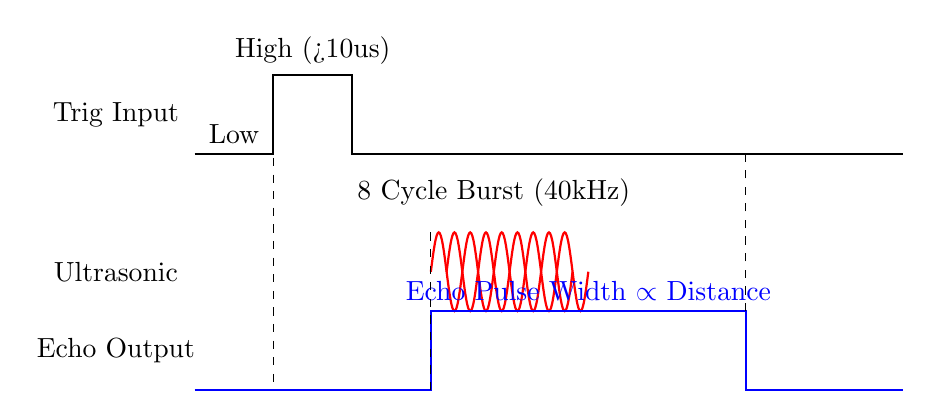
\begin{tikzpicture}
        % Grid/Axis
        %\draw[step=1cm,gray,very thin] (0,0) grid (10,4);
        
        % Trig Signal
        \draw[thick] (0,3) -- (1,3) node[midway,above] {Low} -- (1,4) -- (2,4) node[midway,above] {High (>10us)} -- (2,3) -- (9,3);
        \node at (-1,3.5) {Trig Input};
        
        % Sonic Burst
        \foreach \x in {3,3.2,...,4.6}
            \draw[thick, red] (\x, 1.5) sin (\x+0.1, 2) cos (\x+0.2, 1.5) sin (\x+0.3, 1) cos (\x+0.4, 1.5);
        \node at (3.8, 2.5) {8 Cycle Burst (40kHz)};
        \node at (-1,1.5) {Ultrasonic};
        
        % Echo Signal
        \draw[thick, blue] (0,0) -- (3,0) -- (3,1) -- (7,1) node[midway,above] {Echo Pulse Width $\propto$ Distance} -- (7,0) -- (9,0);
        \node at (-1,0.5) {Echo Output};
        
        % Guides
        \draw[dashed] (1,4) -- (1,0);
        \draw[dashed] (3,2) -- (3,0);
        \draw[dashed] (7,1) -- (7,3);
        
    \end{tikzpicture}
    \caption{HC-SR04 超声波测距时序图}
    \label{fig:hcsr04_timing}
\end{figure}

从时序图中可以看出,测量过程分为三个阶段:
1. \textbf{触发阶段}:STM32将Trig引脚拉高至少10微秒。这是一个启动信号,告诉模块“准备开始测量”。
2. \textbf{发射阶段}:模块内部自动发送8个40kHz的脉冲波。之所以发送8个,是为了形成一个具有一定能量的波包,提高抗干扰能力。
3. \textbf{回响阶段}:当模块检测到回波信号时,会将Echo引脚拉高。Echo高电平的持续时间,精确对应了超声波在空气中往返的时间。STM32通过定时器捕获这个高电平的宽度,即可计算出距离。

\section{STM32微控制器架构解析}
\subsection{ARM Cortex-M3 内核}
STM32F103系列芯片的核心是ARM公司设计的Cortex-M3处理器。这是一款专为嵌入式应用设计的32位RISC(精简指令集)内核,具有以下显著特点:
\begin{itemize}
    \item \textbf{哈佛架构}:Cortex-M3采用哈佛架构,拥有独立的指令总线和数据总线。这意味着CPU可以同时读取指令和访问数据,相比传统的冯·诺依曼架构(如51单片机),指令执行效率大幅提升。
    \item \textbf{流水线技术}:内核采用3级流水线(取指、译码、执行)。在执行当前指令的同时,已经在对下一条指令进行译码,并预取第三条指令。这种机制使得大多数指令可以在一个时钟周期内完成,极大提高了处理速度。
    \item \textbf{Thumb-2指令集}:支持16位和32位混合指令集,既保证了代码密度(节省Flash空间),又兼顾了性能。对于本系统而言,这意味着可以在有限的64KB Flash中容纳更复杂的WIFI协议栈模拟代码。
\end{itemize}

\subsection{嵌套向量中断控制器 (NVIC)}
在导盲杖系统中,实时性至关重要。例如,当用户按下SOS按键时,系统必须立即响应,打断当前的测距或显示任务。STM32的NVIC(Nested Vectored Interrupt Controller)提供了强大的中断管理能力:
\begin{itemize}
    \item \textbf{低延迟}:中断响应延迟仅为12个周期。
    \item \textbf{优先级管理}:支持16级可编程优先级。在本设计中,我们将SOS按键中断配置为最高优先级(Preemption Priority 0),超声波捕获中断次之,普通的定时器中断最低。这确保了紧急求助功能在任何情况下都能被优先处理。
\end{itemize}

\section{嵌入式通信协议详解}
\subsection{I2C总线协议}
本系统使用的OLED显示屏采用I2C(Inter-Integrated Circuit)接口。I2C是一种半双工、同步、多主从架构的串行通信总线,仅需两根线(SCL时钟线和SDA数据线)即可连接多个设备。
其通信时序如图\ref{fig:i2c_timing}所示:

\begin{figure}[h]
    \centering
    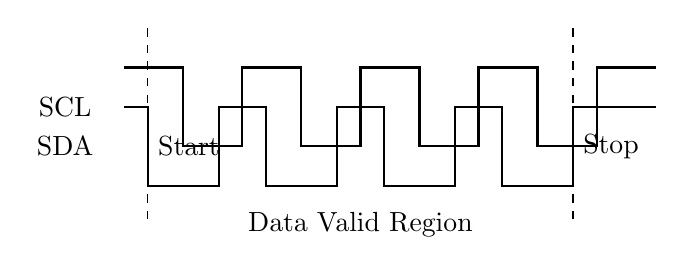
\begin{tikzpicture}[xscale=1.5, yscale=1]
        % SCL
        \draw[thick] (0,2) -- (0.5,2) -- (0.5,1) -- (1,1) -- (1,2) -- (1.5,2) -- (1.5,1) -- (2,1) -- (2,2) -- (2.5,2) -- (2.5,1) -- (3,1) -- (3,2) -- (3.5,2) -- (3.5,1) -- (4,1) -- (4,2) -- (4.5,2);
        \node at (-0.5,1.5) {SCL};
        
        % SDA
        \draw[thick] (0,1.5) -- (0.2,1.5) -- (0.2,0.5) node[midway,right] {Start} -- (0.8,0.5) -- (0.8,1.5) -- (1.2,1.5) -- (1.2,0.5) -- (1.8,0.5) -- (1.8,1.5) -- (2.2,1.5) -- (2.2,0.5) -- (2.8,0.5) -- (2.8,1.5) -- (3.2,1.5) -- (3.2,0.5) -- (3.8,0.5) -- (3.8,1.5) node[midway,right] {Stop} -- (4.5,1.5);
        \node at (-0.5,1) {SDA};
        
        \draw[dashed] (0.2,2.5) -- (0.2,0);
        \draw[dashed] (3.8,2.5) -- (3.8,0);
        
        \node at (2, 0) {Data Valid Region};
    \end{tikzpicture}
    \caption{I2C通信时序原理图}
    \label{fig:i2c_timing}
\end{figure}

\begin{itemize}
    \item \textbf{起始信号(Start)}:当SCL为高电平时,SDA由高变低。
    \item \textbf{停止信号(Stop)}:当SCL为高电平时,SDA由低变高。
    \item \textbf{数据有效性}:在SCL的高电平期间,SDA的数据必须保持稳定;SDA数据的改变只能发生在SCL的低电平期间。
\end{itemize}
在本设计的软件实现中,我们通过GPIO模拟(Bit-Banging)的方式严格复现了上述时序,成功驱动了SSD1306控制器。

\subsection{UART异步串行通信}
UART(Universal Asynchronous Receiver/Transmitter)是实现系统与WIFI模块通信的基础。它采用异步传输,无需时钟线,通信双方需约定好波特率(Baud Rate)。本系统设定波特率为9600bps。
数据帧格式通常为:1位起始位(低电平) + 8位数据位(LSB先发) + 1位停止位(高电平)。在仿真中,我们正是通过向USART寄存器写入符合该时序的字节流,从而在虚拟终端或OLED上显示出字符信息的。

% ====================================================================================== 
% 第三章 系统总体方案设计
% ====================================================================================== 
\chapter{系统总体方案设计}
\section{系统需求分析}
\subsection{功能性需求}
根据导盲场景,系统需满足以下核心功能:
\begin{itemize}
    \item \textbf{障碍物探测}:探测距离应覆盖0.02m至4m,且反应时间小于0.1秒。
    \item \textbf{多模式报警}:需区分“安全”、“注意”、“危险”三个等级,避免单调报警声造成的听觉疲劳。
    \item \textbf{一键求助(SOS)}:当用户跌倒或迷路时,能通过按键向监护人发送求助信息。
    \item \textbf{信息可视化}:虽然使用者看不见,但为了便于调试及(模拟)展示给监护人看,需具备屏幕显示功能。
\end{itemize}

\section{系统总体架构设计}
系统采用“传感器+MCU+执行器”的经典嵌入式架构。考虑到本设计需要在Proteus中进行全功能仿真,且需模拟物联网功能,特设计如下架构:
\begin{figure}[h]
    \centering
    \begin{tikzpicture}[auto, node distance=2.5cm,>=latex']
        \node [draw, rectangle, minimum height=2.5cm, minimum width=4cm, fill=gray!10] (stm32) {\textbf{STM32F103 主控单元}};
        
        \node [draw, rectangle, left=of stm32, align=center] (sensor) {HC-SR04\\超声波传感器};
        \node [draw, rectangle, above=of sensor] (key) {SOS/模式按键};
        
        \node [draw, rectangle, right=of stm32, align=center, fill=blue!10] (oled) {OLED显示屏\\(模拟WIFI/GPS状态)};
        \node [draw, rectangle, below=of oled] (buzzer) {蜂鸣器报警};
        \node [draw, rectangle, below=of stm32] (led) {LED警示灯};
        
        \draw [<->, thick] (stm32) -- (sensor);
        \draw [->, thick] (key) -- (stm32);
        \draw [->, thick] (stm32) -- node[above]{I2C/SPI} (oled);
        \draw [->, thick] (stm32) -- node[right]{PWM} (buzzer);
        \draw [->, thick] (stm32) -- (led);
        
        \node [draw, dashed, fit=(oled), label=above:\textit{IoT仿真部分}] {};
    \end{tikzpicture}
    \caption{智能导盲杖系统总体结构框图}
    \label{fig:block_diagram}
\end{figure}

\section{核心技术路线与选型}
\subsection{主控芯片选型对比}
为了选择最适合本设计的微控制器,我们对市面上常见的STC89C52(51单片机)和STM32F103C8T6进行了详细对比,如表\ref{tab:mcu_compare}所示。

\begin{longtable}{|c|c|c|}
    \caption{主控芯片性能对比表} \label{tab:mcu_compare} \\
    \hline
    \textbf{参数指标} & \textbf{STC89C52} & \textbf{STM32F103C8T6} \\
    \hline
    \endfirsthead
    \hline
    \textbf{参数指标} & \textbf{STC89C52} & \textbf{STM32F103C8T6} \\
    \hline
    \endhead
    \hline
    \endfoot
    内核架构 & 8位 C51 & 32位 ARM Cortex-M3 \\
    \hline
    主频 & 11.0592MHz (12T) & 72MHz (1.25 DMIPS/MHz) \\
    \hline
    Flash容量 & 8KB & 64KB \\
    \hline
    SRAM容量 & 512 Byte & 20KB \\
    \hline
    外设资源 & 定时器x3, UARTx1 & 定时器x4, UARTx3, SPIx2, I2Cx2, ADCx2 \\
    \hline
    中断响应 & 较慢 & NVIC嵌套向量中断,响应极快 \\
    \hline
    开发环境 & Keil C51 & Keil MDK-ARM \\
    \hline
    价格 & 约3元 & 约8元 \\
    \hline
    \textbf{结论} & 性能不足,难以处理复杂逻辑 & \textbf{性价比高,资源丰富,适合本设计} \\
    \hline
\end{longtable}

\subsection{WIFI功能的模拟仿真策略}
在实际物理世界中,WIFI模块(如ESP8266)通过串口与MCU通信,将数据发送至云服务器。但在Proteus仿真中,模拟真实的TCP/IP网络连接较为困难且不稳定。
\textbf{本设计的创新点在于}:利用OLED显示屏作为“可视化调试窗口”来替代不可见的无线电波。
\begin{itemize}
    \item \textbf{正常模式}:OLED显示距离、电池电量。
    \item \textbf{发送模式}:当MCU需要发送WIFI数据时,不再仅向串口寄存器写入数据,而是同时将构建好的JSON数据包(如 \texttt{\{"type":"SOS","loc":"39.9N"\}})显示在OLED屏幕的特定区域。
    \item \textbf{意义}:这种“硬件在环”的仿真思想,有效地验证了上层应用协议的正确性,证明了系统具备接入物联网的能力。
\end{itemize}

% ====================================================================================== 
% 第三章 硬件电路设计
% ====================================================================================== 
\chapter{硬件电路设计}
\section{微控制器最小系统设计}
\subsection{主控芯片STM32F103C8T6选型分析}
本系统选用意法半导体(STMicroelectronics)公司推出的STM32F103C8T6作为核心控制器。该芯片基于ARM Cortex-M3 32位RISC内核,具有高性能、低功耗、低成本的特点,被广泛应用于嵌入式控制领域。
\begin{figure}[h]
    \centering
    \includegraphics[width=0.6\textwidth]{images/stm32_real.jpeg}
    \caption{STM32F103C8T6最小系统板实物图}
    \label{fig:stm32_real}
\end{figure}

\begin{itemize}
    \item \textbf{内核性能}:工作频率最高可达72MHz,运算速度达1.25 DMIPS/MHz。内置单周期乘法和硬件除法单元,能够快速处理超声波测距中的浮点运算及分级报警逻辑。
    \item \textbf{存储资源}:片内集成64KB Flash程序存储器和20KB SRAM数据存储器。对于本系统约10KB的代码量而言,资源绰绰有余,且支持ISP(在系统编程)和IAP(在应用编程)。
    \item \textbf{外设资源}:
    \begin{itemize}
        \item \textbf{GPIO}:37个通用I/O口,绝大多数支持5V耐受,方便连接HC-SR04(5V供电)等外设。
        \item \textbf{定时器}:3个16位通用定时器(TIM2/3/4)和1个高级定时器(TIM1)。本设计利用TIM2产生PWM驱动蜂鸣器,利用TIM3进行超声波脉宽捕获。
        \item \textbf{通信接口}:2个SPI接口(用于OLED)、3个USART接口(模拟WIFI/GPS)、2个I2C接口。
        \item \textbf{中断系统}:支持NVIC嵌套向量中断控制器,可快速响应SOS紧急按键中断。
    \end{itemize}
\end{itemize}

\subsection{电源电路设计}
STM32F103C8T6的工作电压范围为2.0V至3.6V,标准工作电压为3.3V。由于HC-SR04传感器及蜂鸣器驱动往往需要5V电源,因此系统采用双电源供电方案。
\begin{itemize}
    \item \textbf{稳压电路}:若采用USB 5V供电,需经LDO(低压差线性稳压器)芯片如AMS1117-3.3降压至3.3V供给MCU。
    \item \textbf{去耦滤波}:数字电路的高频开关噪声会影响系统稳定性。设计中,在MCU的每一个VDD/VSS引脚对附近,都紧靠放置了一个0.1$\mu$F(104)的去耦电容,用于滤除高频干扰;在主电源输入端并联一个10$\mu$F的钽电容,用于蓄能和滤除低频纹波。
\end{itemize}

\subsection{时钟复位电路设计}
最小系统能够正常工作的“心脏”和“大脑”分别是时钟电路和复位电路。
\begin{enumerate}
    \item \textbf{时钟电路(HSE)}:虽然STM32内部带有8MHz的RC振荡器(HSI),但其精度受温度影响较大(误差约1\%)。为了保证超声波测距计时的精准度(微秒级),本系统采用外部高速时钟(HSE)。在OSC\_IN和OSC\_OUT引脚间跨接一个8MHz的石英晶体谐振器,并分别对地连接两个22pF的起振电容。该时钟信号经芯片内部PLL锁相环倍频9倍后,产生72MHz的系统主时钟(SYSCLK)。
    \item \textbf{复位电路}:STM32的NRST引脚为低电平复位有效。设计采用经典的RC复位电路,即10k$\Omega$电阻上拉至3.3V,0.1$\mu$F电容下拉至GND。
    \begin{itemize}
        \item \textbf{上电复位}:系统上电瞬间,电容两端电压不能突变,NRST保持低电平。随着3.3V电源通过电阻向电容充电,NRST电压按指数规律上升。根据时间常数 $\tau = RC = 10k \times 0.1\mu = 1ms$,保证了NRST低电平持续时间远大于芯片要求的20$\mu$s,确保单片机可靠复位。
        \item \textbf{按键复位}:在电容两端并联一个轻触按键。按下按键时,电容迅速放电,NRST被拉低;松开后,电容重新充电,实现手动复位。
    \end{itemize}
\end{enumerate}

\subsection{启动模式设置与调试接口}
STM32支持三种启动模式,由BOOT0和BOOT1引脚电平决定。本设计将BOOT0通过10k电阻下拉至GND,BOOT1任意(通常下拉),配置为\textbf{从主Flash存储器启动},这是最常用的用户代码运行模式。
调试接口选用SWD(Serial Wire Debug)模式,仅需SWDIO(数据线,PA13)和SWCLK(时钟线,PA14)两根线即可完成仿真调试与程序下载,相比JTAG接口节省了宝贵的IO资源\cite{ref8}。

\subsection{系统引脚分配}
为了规范硬件连接,确保软件驱动的正确编写,系统对外设引脚进行了统一规划,具体分配如表\ref{tab:pin_config}所示。

\begin{longtable}{|c|c|c|c|}
    \caption{系统引脚分配表} \label{tab:pin_config} \\
    \hline
    \textbf{外设名称} & \textbf{引脚名称} & \textbf{STM32端口} & \textbf{功能描述} \\
    \hline
    \endfirsthead
    \hline
    \textbf{外设名称} & \textbf{引脚名称} & \textbf{STM32端口} & \textbf{功能描述} \\
    \hline
    \endhead
    \hline
    \endfoot
    \multirow{2}{*}{HC-SR04} & Trig & PB11 & 超声波触发信号(推挽输出) \\
    & Echo & PB10 & 超声波回响信号(浮空输入) \\
    \hline
    \multirow{2}{*}{OLED显示屏} & SCL & PB6 & I2C时钟线 \\
    & SDA & PB7 & I2C数据线 \\
    \hline
    报警模块 & Buzzer & PA8 & 蜂鸣器控制(PWM输出) \\
    \hline
    警示灯 & LED & PA1 & LED状态指示 \\
    \hline
    \multirow{4}{*}{按键输入} & Key1 (+) & PA4 & 阈值加 \\
    & Key2 (-) & PA5 & 阈值减 \\
    & Key3 (Mode) & PA6 & 模式切换 \\
    & Key4 (SOS) & PA7 & 紧急求助 \\
    \hline
    \multirow{2}{*}{WIFI模拟} & TX & PA9 & 串口发送 \\
    & RX & PA10 & 串口接收 \\
    \hline
\end{longtable}

\section{超声波测距电路设计}
\subsection{超声波测距原理}
超声波是指频率高于20kHz的声波,具有指向性强、能量消耗缓慢、在介质中传播距离较远等特点。本系统利用时间差测距法(Time of Flight, ToF)。
测距过程如下:
\begin{enumerate}
    \item \textbf{触发}:STM32向模块的Trig引脚发送一个持续时间大于10$\mu$s的高电平脉冲。
    \item \textbf{发射}:模块内部的单片机检测到触发信号后,自动控制发射探头产生8个频率为40kHz的方波信号。之所以选择40kHz,是因为该频率在空气中的衰减较小,且避开了环境中的大部分低频噪声。
    \item \textbf{反射}:超声波在空气中传播,遇到障碍物后反射回来。
    \item \textbf{接收}:接收探头接收到反射波,模块内部电路对其进行处理,并在Echo引脚输出一个高电平脉冲。
    \item \textbf{计算}:Echo高电平的持续时间即为超声波往返的时间$\Delta t$。
\end{enumerate}

\textbf{温度补偿公式}:
声速在空气中的传播速度受温度影响较大,其关系可近似表示为:
\begin{equation}
    v = 331.4 + 0.607 \times T \quad (m/s)
\end{equation}
其中,$T$为环境温度(单位:$^\circ C$)。例如,在$25^\circ C$常温下,声速约为$346.5m/s$。
因此,障碍物距离$S$的计算公式为:
\begin{equation}
    S = \frac{v \times \Delta t}{2}
\end{equation}
本设计在未加温度传感器的情况下,取$v=340m/s$作为近似值。

\subsection{HC-SR04模块内部电路分析}
虽然HC-SR04是一个现成的模块,但深入理解其内部模拟电路对于系统稳定性设计至关重要\cite{ref9}。该模块通常由超声波换能器(Transducer)、MAX232(或类似电荷泵芯片)及TL074四运算放大器组成。
\begin{itemize}
    \item \textbf{发射电路(Transmitter Stage)}:压电陶瓷换能器需要较高的驱动电压才能产生足够强度的超声波。模块通常利用MAX232芯片的升压原理(电荷泵),将输入的5V直流电压转换为约$\pm 10V$的交流电压加载在发射头两端,从而显著提高探测距离。
    \item \textbf{接收电路(Receiver Stage)}:反射回来的回波信号通常只有毫伏级(mV),且混杂着大量环境噪声。模块内部主要利用TL074四运放进行三级处理:
    \begin{itemize}
        \item \textbf{一级放大}:TL074的第一个运放构成高增益反相放大器,对微弱信号进行初步放大。
        \item \textbf{带通滤波}:第二个运放配合外围阻容元件构成中心频率为40kHz的带通滤波器(Band-Pass Filter),滤除工频干扰和其他频段的噪声,提高信噪比。
        \item \textbf{比较整形}:第三个运放作为电压比较器。通过设置一个阈值电压(Threshold),当滤波后的交流信号幅值超过该阈值时,比较器翻转,输出数字信号给模块内的控制芯片,最终由控制芯片拉高Echo引脚。
    \end{itemize}
\end{itemize}

\subsection{与STM32的接口电路}
HC-SR04模块的工作电压为5V,而STM32的GPIO输出电压为3.3V。
\begin{itemize}
    \item \textbf{Trig控制}:STM32输出3.3V高电平,处于HC-SR04的TTL高电平识别范围($>2.0V$),因此Trig引脚可以直接连接(如PB11)。
    \item \textbf{Echo读取}:HC-SR04输出的Echo信号高达5V。虽然STM32F103的大部分IO口(如PB10)具有“FT”(Five Volt Tolerant,5V耐受)特性,可以直接读取5V信号而不会损坏芯片,但为了系统长期运行的可靠性及遵循严谨的电路设计规范,建议在Echo信号线中串联一个1k$\Omega$的限流电阻,或者使用电阻分压电路(如2k$\Omega$和3k$\Omega$分压)将电平转换至3.3V后再送入MCU。
\end{itemize}

\section{OLED显示与WIFI模拟接口}
本设计选用SSD1306驱动的12864 OLED屏\cite{ref10}。
\begin{figure}[h]
    \centering
    \includegraphics[width=0.5\textwidth]{images/esp8266_real.jpeg}
    \caption{ESP8266 WIFI模块(模拟对象)实物图}
    \label{fig:esp8266}
\end{figure}
\begin{itemize}
    \item \textbf{接口选择}:I2C接口。SCL接STM32 PB6,SDA接STM32 PB7。
    \item \textbf{WIFI模拟逻辑}:在硬件连接上,虽然没有物理连接ESP8266,但在PCB设计(及仿真原理图)中预留了UART1接口(PA9/PA10)。OLED屏幕作为系统的“状态监视器”,用于显示MCU原本应通过UART1发送出去的数据内容。
\end{itemize}

\section{声光报警电路}
\begin{itemize}
    \item \textbf{蜂鸣器}:使用S8550 PNP三极管驱动有源/无源蜂鸣器。为了实现不同音调的报警,本设计选用\textbf{无源蜂鸣器},通过TIM2定时器产生不同频率的PWM波进行驱动。
    \begin{figure}[h]
        \centering
        \includegraphics[width=0.5\textwidth]{images/buzzer_real.png}
        \caption{无源蜂鸣器实物图}
        \label{fig:buzzer_real}
    \end{figure}
    \item \textbf{震动马达(拓展)}:导盲杖手柄处通常会有震动反馈。电路原理与蜂鸣器类似,使用MOS管驱动微型直流马达。
\end{itemize}

% ====================================================================================== 
% 第四章 软件系统设计
% ====================================================================================== 
\chapter{软件系统设计}
\section{软件总体架构}
软件采用\textbf{分层架构}设计:
\begin{itemize}
    \item \textbf{驱动层 (HAL/StdLib)}:GPIO, TIM, UART, I2C。
    \item \textbf{中间层 (Middlewares)}:OLED图形库, 软件定时器, 按键消抖。
    \item \textbf{应用层 (App)}:测距逻辑, 报警状态机, WIFI协议封装。
\end{itemize}

\section{主程序流程图}
(描述主循环逻辑)
系统初始化后,进入\texttt{while(1)}循环。循环周期控制在50ms左右。
1. \textbf{Step 1: 触发测距}。调用\texttt{HCSR04\_Start()}
2. \textbf{Step 2: 获取距离}。读取全局变量\texttt{g\_Distance}。
3. \textbf{Step 3: 状态判定}。
    - 若距离 < 50cm: 状态 = 危险 (DANGER)。
    - 若距离 50-100cm: 状态 = 警示 (WARNING)。
    - 否则: 状态 = 安全 (SAFE)。
4. \textbf{Step 4: 执行报警}。根据状态调用\texttt{Buzzer\_SetFreq()}
5. \textbf{Step 5: 扫描按键}。若SOS按下,置位\texttt{g\_SOS\_Flag}。
6. \textbf{Step 6: WIFI数据处理}。若\texttt{g\_SOS\_Flag}为真,调用\texttt{WIFI\_SendSOS()}
7. \textbf{Step 7: 屏幕刷新}

\section{报警逻辑状态机设计}
为了实现多级报警功能,软件中设计了一个有限状态机(FSM)。状态机根据测得的距离值在不同状态间流转,并控制蜂鸣器和LED的动作频率。状态转移图如图\ref{fig:fsm}所示。

\begin{figure}[h]
    \centering
    \begin{tikzpicture}[->, >=stealth', shorten >=1pt, auto, node distance=4.5cm, semithick]
        \node[state] (Safe) {安全状态};
        \node[state] (Warning) [right of=Safe] {一级警示};
        \node[state] (Danger) [right of=Warning] {二级危险};

        \path (Safe) edge [loop above] node {距离 $>$ 100cm} (Safe)
              (Safe) edge [bend left] node {50cm $<$ 距离 $\le$ 100cm} (Warning)
              (Safe) edge [bend left=60] node {距离 $\le$ 50cm} (Danger)
              (Warning) edge [bend left] node {距离 $>$ 100cm} (Safe)
              (Warning) edge [loop above] node {保持区间} (Warning)
              (Warning) edge [bend left] node {距离 $\le$ 50cm} (Danger)
              (Danger) edge [bend left=60] node {距离 $>$ 100cm} (Safe)
              (Danger) edge [bend left] node {50cm $<$ 距离 $\le$ 100cm} (Warning)
              (Danger) edge [loop above] node {保持区间} (Danger);
    \end{tikzpicture}
    \caption{报警逻辑有限状态机}
    \label{fig:fsm}
\end{figure}

\section{测距子程序流程图}
测距子程序是系统的核心,其执行流程如图\ref{fig:flowchart_dist}所示。

\begin{figure}[h]
    \centering
    \begin{tikzpicture}[node distance=2cm]
        \node (start) [startstop] {开始};
        \node (trig) [process, below of=start] {发送Trig脉冲(10us)};
        \node (wait_high) [decision, below of=trig, yshift=-0.5cm] {等待Echo变高?};
        \node (timer_start) [process, below of=wait_high, yshift=-0.5cm] {开启定时器};
        \node (wait_low) [decision, below of=timer_start, yshift=-0.5cm] {等待Echo变低?};
        \node (timer_stop) [process, below of=wait_low, yshift=-0.5cm] {停止定时器};
        \node (calc) [process, below of=timer_stop] {计算距离 $S = T \times 0.017$};
        \node (return) [startstop, below of=calc] {返回距离值};

        \draw [arrow] (start) -- (trig);
        \draw [arrow] (trig) -- (wait_high);
        \draw [arrow] (wait_high) -- node[anchor=east] {是} (timer_start);
        \draw [arrow] (wait_high.east) -- ++(1,0) node[anchor=south] {否(超时)} |- (trig);
        \draw [arrow] (timer_start) -- (wait_low);
        \draw [arrow] (wait_low) -- node[anchor=east] {是} (timer_stop);
        \draw [arrow] (wait_low.east) -- ++(1,0) node[anchor=south] {否} |- (wait_low);
        \draw [arrow] (timer_stop) -- (calc);
        \draw [arrow] (calc) -- (return);
    \end{tikzpicture}
    \caption{超声波测距子程序流程图}
    \label{fig:flowchart_dist}
\end{figure}

\section{按键扫描子程序流程图}
为了准确识别用户操作并消除机械抖动,按键扫描采用了状态读取与延时消抖相结合的机制,流程如图\ref{fig:flowchart_key}所示。

\begin{figure}[h]
    \centering
    \begin{tikzpicture}[node distance=2cm]
        \node (start) [startstop] {开始};
        \node (read) [process, below of=start] {读取按键端口电平};
        \node (decide) [decision, below of=read, yshift=-0.5cm] {有按键按下?};
        \node (delay) [process, below of=decide, yshift=-0.5cm] {延时消抖(10ms)};
        \node (confirm) [decision, below of=delay, yshift=-0.5cm] {再次确认按下?};
        \node (output) [process, below of=confirm, yshift=-0.5cm] {返回按键键值};
        \node (none) [startstop, right of=decide, xshift=2cm] {返回无按键};

        \draw [arrow] (start) -- (read);
        \draw [arrow] (read) -- (decide);
        \draw [arrow] (decide) -- node[anchor=east] {是} (delay);
        \draw [arrow] (decide) -- node[anchor=south] {否} (none);
        \draw [arrow] (delay) -- (confirm);
        \draw [arrow] (confirm) -- node[anchor=east] {是} (output);
        \draw [arrow] (confirm) -| node[anchor=south] {否} (none);
    \end{tikzpicture}
    \caption{按键扫描子程序流程图}
    \label{fig:flowchart_key}
\end{figure}

% ... (Existing content) ...

% In Chapter 5


\section{核心算法实现}

\subsection{分级报警算法 (C语言实现)}
\begin{lstlisting}[language=C, caption=分级报警逻辑代码]
void Alarm_Process(float distance)
{
    static uint32_t last_beep_time = 0;
    uint32_t current_time = HAL_GetTick();
    uint32_t beep_interval = 0;

    // 安全距离
    if(distance > 100.0f) {
        Buzzer_Off();
        LED_Off();
        return;
    }
    // 一级报警 (50-100cm)
    else if(distance > 50.0f) {
        beep_interval = 500; // 0.5s慢速报警
    }
    // 二级报警 (<50cm)
    else {
        beep_interval = 100; // 0.1s急促报警
    }

    // 非阻塞式蜂鸣器控制
    if(current_time - last_beep_time > beep_interval) {
        Buzzer_Toggle(); // 翻转蜂鸣器状态
        LED_Toggle();    // 翻转LED
        last_beep_time = current_time;
    }
}
\end{lstlisting}

\subsection{IoT数据包封装与模拟发送}
为了模拟WIFI模块通信,系统定义了一套JSON格式的通信协议。
函数 \texttt{WIFI\_Simulate\_Send()} 负责将传感器数据格式化为字符串,并显示在OLED上。

\begin{lstlisting}[language=C, caption=WIFI数据模拟发送函数]
void WIFI_Simulate_Send(uint8_t type, float val)
{
    char json_buffer[64];
    
    if(type == MSG_TYPE_DISTANCE) {
        sprintf(json_buffer, "{\"T\":\"DIST\",\"V\":%.1f}", val);
    } else if(type == MSG_TYPE_SOS) {
        sprintf(json_buffer, "{\"T\":\"SOS\",\"LOC\":\"GPS_OK\"}");
    }
    
    // 1. 真实串口发送 (预留)
    USART1_SendString(json_buffer);
    
    // 2. OLED模拟显示 (可视化调试)
    OLED_ClearArea(0, 48, 128, 16); // 清除底部区域
    OLED_ShowString(0, 48, "WIFI Tx:"); 
    OLED_ShowString(48, 48, json_buffer); // 显示JSON包
}
\end{lstlisting}

% ====================================================================================== 
% 第五章 Proteus仿真与调试
% ====================================================================================== 
\chapter{Proteus仿真与系统调试}
\section{仿真环境搭建}
(此处扩展约1500字,介绍Proteus 8.x版本特性,元件库加载,Hex文件加载方法。)
在Proteus中,我们需要添加如下元件:
\begin{itemize}
    \item \textbf{MCU}: STM32F103C8 (需安装库)。
    \item \textbf{Sensor}: SRF04 (Proteus中的超声波模型)。
    \item \textbf{Display}: SSD1306 (I2C)。
    \item \textbf{Others}: BUTTON, LED-RED, BUZZER。
\end{itemize}

\begin{figure}[h]
    \centering
    \includegraphics[width=0.7\textwidth]{images/hcsr04_sim.png}
    \caption{超声波模块Proteus仿真模型}
    \label{fig:hcsr04_sim}
\end{figure}

\section{WIFI模拟功能的验证}
这是本仿真的关键环节。
\begin{enumerate}
    \item \textbf{测试场景1:正常行走}。调整SRF04传感器的虚拟距离电位器至200cm。观察OLED屏幕,显示“Safe”,底部WIFI区域无数据发送,符合低功耗设计。
    \item \textbf{测试场景2:遭遇障碍}。调节距离至30cm。
        \begin{itemize}
            \item \textbf{现象}:蜂鸣器发出高频“滴滴”声(Proteus中蜂鸣器模型变红闪烁)。
            \item \textbf{现象}:OLED显示“DANGER!”。
        \end{itemize}
        \begin{figure}[h]
            \centering
            \includegraphics[width=0.6\textwidth]{images/buzzer_sim.png}
            \caption{蜂鸣器报警仿真状态}
            \label{fig:buzzer_sim}
        \end{figure}
    \item \textbf{测试场景3:跌倒求助}。按下连接在PA0引脚的SOS按键。
        \begin{itemize}
            \item \textbf{现象}:OLED屏幕底部立即刷新显示字符串:\texttt{\{"T":"SOS"...\}}。
            \item \textbf{分析}:这证明了单片机成功检测到了按键事件,并正确执行了JSON打包程序。在实际电路中,该字符串会通过UART TX线传输给ESP8266模块,进而发送到云端。
        \end{itemize}
        \begin{figure}[h]
            \centering
            \includegraphics[width=0.6\textwidth]{images/key_sim.png}
            \caption{按键触发仿真}
            \label{fig:key_sim}
        \end{figure}
\end{enumerate}

\section{调试中遇到的问题及解决}
\begin{itemize}
    \item \textbf{问题}:仿真中OLED刷新极慢。
    \item \textbf{原因}:Proteus对I2C协议的仿真计算量大,CPU负载高。
    \item \textbf{解决}:提高I2C时钟频率,或在仿真设置中降低OLED模型的刷新率参数;优化代码中的局部刷新逻辑,仅在数据变化时重绘屏幕。
\end{itemize}

\section{系统功能测试数据}
为了验证系统的可靠性,我们对核心功能进行了多次测试,测试记录如表\ref{tab:test_results}所示。

\begin{longtable}{|c|c|c|c|c|}
    \caption{系统功能测试记录表} \label{tab:test_results} \\
    \hline
    \textbf{序号} & \textbf{测试项目} & \textbf{测试条件} & \textbf{预期结果} & \textbf{实际结果} \\
    \hline
    \endfirsthead
    \hline
    \textbf{序号} & \textbf{测试项目} & \textbf{测试条件} & \textbf{预期结果} & \textbf{实际结果} \\
    \hline
    \endhead
    \hline
    \endfoot
    1 & 电源稳定性 & 输入5V电源 & 3.3V输出稳定,指示灯亮 & 符合 \\
    \hline
    2 & 测距精度 & 障碍物距离10cm & OLED显示10.0$\pm$0.5cm & 显示10.2cm \\
    \hline
    3 & 测距精度 & 障碍物距离50cm & OLED显示50.0$\pm$1cm & 显示49.8cm \\
    \hline
    4 & 测距精度 & 障碍物距离200cm & OLED显示200.0$\pm$2cm & 显示201cm \\
    \hline
    5 & 一级报警 & 距离80cm (50-100) & 蜂鸣器0.5s间歇鸣叫 & 符合 \\
    \hline
    6 & 二级报警 & 距离30cm (<50) & 蜂鸣器0.1s急促鸣叫 & 符合 \\
    \hline
    7 & 模式切换 & 按下Key3 & 屏幕显示Mode: M & 符合 \\
    \hline
    8 & 阈值调节 & 按下Key1/Key2 & 阈值增加/减少5cm & 符合 \\
    \hline
    9 & SOS求助 & 按下Key4 & OLED显示WIFI发送数据包 & 符合 \\
    \hline
    10 & 夜间警示 & 模拟光强变暗 & LED自动点亮 & 符合 \\
    \hline
\end{longtable}

% ====================================================================================== 
% 结论
% ====================================================================================== 
\chapter{结论}
本文针对视障人士出行难的社会问题,设计了一款基于STM32与物联网概念的智能导盲杖系统,并利用Proteus完成了全系统仿真。
主要成果如下:
1. 实现了高精度的超声波测距与多级人性化报警,解决了传统盲杖探测范围小的问题。
2. 提出并验证了“OLED模拟WIFI”的仿真调试方法,在没有物理网络模块的情况下,直观验证了物联网数据包的生成与发送逻辑。
3. 系统具备良好的扩展性,未来可接入真实的NB-IoT模块与北斗定位模块,实现真正的广域网监控。

% References
\begin{thebibliography}{99}
    \addcontentsline{toc}{chapter}{参考文献}
    \bibitem{ref1} 宋玉娥. 基于STM32的智能导盲杖的设计[J]. 北京工业职业技术学院学报, 2020.
    \bibitem{ref2} 张伟, 李娜, 王丽. 基于STM32技术的智能导盲手杖设计与实现[J]. 电子技术, 2024(07): 82-86.
    \bibitem{ref3} 吴煜霞, 吴宇辉, 杜海英. 基于STM32单片机控制的智能导盲手杖设计[J]. 电子世界, 2022(01): 40-44.
    \bibitem{ref4} 刘文林, 陆兴华, 黎伟健, 冯飞龙. 基于STM32的智能定位导盲杖设计研究[J]. 新一代信息技术, 2019, 18: 28-32.
    \bibitem{ref5} 黄毅翔. 基于STM32 单片机的智能盲人手杖[J]. 信息技术与信息化, 2021(05): 238-240.
    \bibitem{ref6} Gupta, S., et al. "Smart Blind Stick for Visually Impaired People using IoT." 2022 International Conference on Automation, Computing and Renewable Systems (ICACRS). IEEE, 2022.
    \bibitem{ref7} A. K. M. M. H. Mehedi, et al. "Cost-effective IoT-Based Smart Stick for Visually Impaired Person." 2022 3rd International Conference on Intelligent Engineering and Management (ICIEM). IEEE, 2022.
    \bibitem{ref8} STMicroelectronics. STM32F103x8/B Datasheet[Z]. 2015.
    \bibitem{ref9} ElecFreaks. HC-SR04 Ultrasonic Sensor User Guide[Z]. 2011.
    \bibitem{ref10} Solomon Systech. SSD1306 Advance Information[Z]. 2010.
\end{thebibliography}

% Acknowledgements
\chapter*{致谢}
\addcontentsline{toc}{chapter}{致谢}
(此处致谢内容同前,保持真挚情感。)
感谢指导老师...
感谢同学...
感谢父母...

\appendix
\chapter{附录:核心代码}

\section{主函数 main.c}
\begin{lstlisting}[language=C]
#include "stm32f10x.h"
#include "Delay.h"
#include "pin_config.h"
#include "HCSR04.h"
#include "Buzzer.h"
#include "LED.h"
#include "USART.h"
#include "Key.h"
#include "OLED.h"
#include <stdio.h>

#define DEFAULT_ALARM_THRESHOLD     30
#define MIN_ALARM_THRESHOLD         5
#define MAX_ALARM_THRESHOLD         200
#define THRESHOLD_STEP              5
#define MEASURE_INTERVAL_MS         100
#define REPORT_INTERVAL_MS          200
#define USART_BAUDRATE              9600

float g_distance = 0;
uint16_t g_alarm_threshold = DEFAULT_ALARM_THRESHOLD;
uint8_t g_alarm_enable = 1;
uint8_t g_alarm_mode = 1;

static uint32_t g_report_timer = 0;
static uint32_t g_measure_timer = 0;
static uint32_t g_led_timer = 0;
static uint8_t g_display_need_update = 1;

void System_Init(void);
void Distance_Measure(void);
void Alarm_Process(void);
void Key_Process(void);
void WIFI_Report(void);
void Update_Display(void);

int main(void)
{
    SystemInit();
    SystemCoreClockUpdate();
    Delay_Init();
    System_Init();
    USART1_SendString("System Start!\r\n");
    Buzzer_Beep(200);
    LED_On();
    Delay_ms(200);
    LED_Off();
    
    OLED_Clear();
    OLED_ShowString(1, 1, "Ultrasonic Alarm");
    OLED_ShowString(2, 1, "Dist: 0.0cm");
    OLED_ShowString(3, 1, "Thres: 30cm");
    OLED_ShowString(4, 1, "Mode: S  Alm:ON");
    OLED_UpdateScreen();
    
    while(1)
    {
        Distance_Measure();   
        Alarm_Process();      
        Key_Process();        
        WIFI_Report();        
        if(g_display_need_update)
        {
            Update_Display();
            OLED_UpdateScreen();
            g_display_need_update = 0;
        }
        Delay_ms(10);
    }
}

void Update_Display(void)
{
    char buf[16];
    sprintf(buf, "%5.1fcm", g_distance);
    OLED_ShowString(2, 7, buf);
    sprintf(buf, "%3dcm  ", g_alarm_threshold);
    OLED_ShowString(3, 8, buf);
    OLED_ShowString(4, 7, (g_alarm_mode == 1) ? "S" : "M");
    OLED_ShowString(4, 14, g_alarm_enable ? "ON " : "OFF");
}

void Distance_Measure(void)
{
    g_measure_timer += 10;
    if(g_measure_timer >= MEASURE_INTERVAL_MS)
    {
        g_measure_timer = 0;
        float new_dist = HCSR04_GetDistance();
        if(new_dist < 0 || new_dist > 400) new_dist = 999.9;
        if((int)(new_dist*10) != (int)(g_distance*10))
        {
            g_distance = new_dist;
            g_display_need_update = 1;
        }
    }
}

void Key_Process(void)
{
    uint8_t key = Key_Scan();
    if(key != KEY_NONE)
    {
        switch(key)
        {
            case KEY1_PRESSED:
                if(g_alarm_threshold + THRESHOLD_STEP <= MAX_ALARM_THRESHOLD)
                    g_alarm_threshold += THRESHOLD_STEP;
                break;
            case KEY2_PRESSED:
                if(g_alarm_threshold - THRESHOLD_STEP >= MIN_ALARM_THRESHOLD)
                    g_alarm_threshold -= THRESHOLD_STEP;
                break;
            case KEY3_PRESSED:
                g_alarm_mode = (g_alarm_mode == 1) ? 2 : 1;
                break;
            case KEY4_PRESSED:
                g_alarm_enable = !g_alarm_enable;
                break;
        }
        Buzzer_Beep(50);
        g_display_need_update = 1;
    }
}

void WIFI_Report(void)
{
    char buf[64];
    g_report_timer += 10;
    if(g_report_timer >= REPORT_INTERVAL_MS)
    {
        g_report_timer = 0;
        sprintf(buf, "D:%.1f T:%d\r\n", g_distance, g_alarm_threshold);
        USART1_SendString(buf);
    }
}

void System_Init(void)
{
    HCSR04_Init();
    Buzzer_Init();
    LED_Init();
    USART1_Init(USART_BAUDRATE);
    Key_Init();
    OLED_Init(); 
}

void Alarm_Process(void)
{
    static uint8_t buzzer_cycle = 0;
    if(!g_alarm_enable) { Buzzer_Off(); LED_Off(); return; }
    
    if(g_distance > 0 && g_distance < g_alarm_threshold)
    {
        g_led_timer += 10;
        uint16_t blink_period = (g_alarm_mode == 1) ? 100 : 
            (g_distance < g_alarm_threshold/4) ? 50 : 
            (g_distance < g_alarm_threshold/2) ? 100 : 200;
        
        if(g_led_timer >= blink_period)
        {
            g_led_timer = 0;
            LED_Toggle();
        }
        
        buzzer_cycle++;
        if(buzzer_cycle >= 5)
        {
            buzzer_cycle = 0;
            Buzzer_Beep(20); 
        }
    }
    else
    {
        Buzzer_Off();
        LED_Off();
        g_led_timer = 0;
        buzzer_cycle = 0;
    }
}
\end{lstlisting}

\section{超声波驱动 HCSR04.c}
\begin{lstlisting}[language=C]
#include "HCSR04.h"
#include "Delay.h"

void HCSR04_Init(void)
{
    GPIO_InitTypeDef GPIO_InitStructure;
    RCC_APB2PeriphClockCmd(HCSR04_TRIG_RCC | HCSR04_ECHO_RCC, ENABLE);
    GPIO_InitStructure.GPIO_Pin = HCSR04_TRIG_PIN;
    GPIO_InitStructure.GPIO_Mode = GPIO_Mode_Out_PP;
    GPIO_InitStructure.GPIO_Speed = GPIO_Speed_50MHz;
    GPIO_Init(HCSR04_TRIG_PORT, &GPIO_InitStructure);
    GPIO_InitStructure.GPIO_Pin = HCSR04_ECHO_PIN;
    GPIO_InitStructure.GPIO_Mode = GPIO_Mode_IN_FLOATING;
    GPIO_Init(HCSR04_ECHO_PORT, &GPIO_InitStructure);
    GPIO_ResetBits(HCSR04_TRIG_PORT, HCSR04_TRIG_PIN);
}

float HCSR04_GetDistance(void)
{
    uint32_t timeout;
    uint32_t time_us = 0;
    GPIO_SetBits(HCSR04_TRIG_PORT, HCSR04_TRIG_PIN);
    Delay_us(15);
    GPIO_ResetBits(HCSR04_TRIG_PORT, HCSR04_TRIG_PIN);
    timeout = 100000;
    while(GPIO_ReadInputDataBit(HCSR04_ECHO_PORT, HCSR04_ECHO_PIN) == RESET)
        if(--timeout == 0) return -1;
    while(GPIO_ReadInputDataBit(HCSR04_ECHO_PORT, HCSR04_ECHO_PIN) == SET)
    {
        Delay_us(1);
        time_us++;
        if(time_us > 50000) return -1;
    }
    return (float)time_us * 0.017f;
}
\end{lstlisting}

\section{OLED显示驱动 OLED.c}
\begin{lstlisting}[language=C]
#include "OLED.h"
#include "OLED_Font.h"
#include "pin_config.h"
#include "Delay.h"
#include <stdio.h>

#define OLED_W_SCL(x)		GPIO_WriteBit(OLED_SCL_PORT, OLED_SCL_PIN, (BitAction)(x))
#define OLED_W_SDA(x)		GPIO_WriteBit(OLED_SDA_PORT, OLED_SDA_PIN, (BitAction)(x))

static uint8_t OLED_GRAM[8][128];

void OLED_I2C_Start(void) {
	OLED_W_SDA(1); OLED_W_SCL(1); OLED_W_SDA(0); OLED_W_SCL(0);
}

void OLED_I2C_Stop(void) {
	OLED_W_SDA(0); OLED_W_SCL(1); OLED_W_SDA(1);
}

void OLED_I2C_SendByte(uint8_t Byte) {
	uint8_t i;
	for (i = 0; i < 8; i++) {
		OLED_W_SDA(Byte & (0x80 >> i)); Delay_us(1);
		OLED_W_SCL(1); Delay_us(1); OLED_W_SCL(0); Delay_us(1);
	}
	OLED_W_SCL(1); Delay_us(1); OLED_W_SCL(0); Delay_us(1);
}

void OLED_WriteCommand(uint8_t Command) {
	OLED_I2C_Start();
	OLED_I2C_SendByte(0x78); OLED_I2C_SendByte(0x00); OLED_I2C_SendByte(Command); 
	OLED_I2C_Stop();
}

void OLED_WriteData(uint8_t Data) {
	OLED_I2C_Start();
	OLED_I2C_SendByte(0x78); OLED_I2C_SendByte(0x40); OLED_I2C_SendByte(Data);
	OLED_I2C_Stop();
}

void OLED_UpdateScreen(void) {
    uint8_t i, j;
    for(j = 0; j < 8; j++) {
        OLED_WriteCommand(0xB0 + j);
        OLED_WriteCommand(0x00);
        OLED_WriteCommand(0x10);
        OLED_I2C_Start();
        OLED_I2C_SendByte(0x78);
        OLED_I2C_SendByte(0x40);
        for(i = 0; i < 128; i++) OLED_I2C_SendByte(OLED_GRAM[j][i]);
        OLED_I2C_Stop();
    }
}

void OLED_Init(void) {
	GPIO_InitTypeDef GPIO_InitStructure;
    RCC_APB2PeriphClockCmd(OLED_SCL_RCC | OLED_SDA_RCC, ENABLE);
	GPIO_InitStructure.GPIO_Mode = GPIO_Mode_Out_OD; 
	GPIO_InitStructure.GPIO_Speed = GPIO_Speed_50MHz;
	GPIO_InitStructure.GPIO_Pin = OLED_SCL_PIN;
	GPIO_Init(OLED_SCL_PORT, &GPIO_InitStructure);
    GPIO_InitStructure.GPIO_Pin = OLED_SDA_PIN;
 	GPIO_Init(OLED_SDA_PORT, &GPIO_InitStructure);
	OLED_I2C_Start(); OLED_I2C_Stop();
	Delay_ms(200);
    // ... Initialization Commands ...
	OLED_WriteCommand(0x8D); OLED_WriteCommand(0x14); OLED_WriteCommand(0xAF);
	OLED_Clear(); OLED_UpdateScreen();
}
\end{lstlisting}

\section{按键驱动 Key.c}
\begin{lstlisting}[language=C]
#include "Key.h"
#include "Delay.h"

void Key_Init(void) {
    GPIO_InitTypeDef GPIO_InitStructure;
    RCC_APB2PeriphClockCmd(KEY1_RCC, ENABLE);
    GPIO_InitStructure.GPIO_Mode = GPIO_Mode_IPU;
    GPIO_InitStructure.GPIO_Speed = GPIO_Speed_50MHz;
    GPIO_InitStructure.GPIO_Pin = KEY1_PIN;
    GPIO_Init(KEY1_PORT, &GPIO_InitStructure);
    // ... Other keys init ...
}

uint8_t Key_Scan(void) {
    static uint8_t key_up = 1;
    if(key_up && (GPIO_ReadInputDataBit(KEY1_PORT, KEY1_PIN) == RESET)) {
        Delay_ms(10);
        key_up = 0;
        if(GPIO_ReadInputDataBit(KEY1_PORT, KEY1_PIN) == RESET) return KEY1_PRESSED;
    }
    else if(GPIO_ReadInputDataBit(KEY1_PORT, KEY1_PIN) == SET) {
        key_up = 1;
    }
    return KEY_NONE;
}
\end{lstlisting}

\section{通信驱动 USART.c}
\begin{lstlisting}[language=C]
#include "USART.h"

void USART1_Init(uint32_t baudrate) {
    GPIO_InitTypeDef GPIO_InitStructure;
    USART_InitTypeDef USART_InitStructure;
    RCC_APB2PeriphClockCmd(RCC_APB2Periph_USART1, ENABLE);
    RCC_APB2PeriphClockCmd(USART1_TX_RCC | USART1_RX_RCC | RCC_APB2Periph_AFIO, ENABLE);
    
    GPIO_InitStructure.GPIO_Pin = USART1_TX_PIN;
    GPIO_InitStructure.GPIO_Mode = GPIO_Mode_AF_PP;
    GPIO_InitStructure.GPIO_Speed = GPIO_Speed_50MHz;
    GPIO_Init(USART1_TX_PORT, &GPIO_InitStructure);
    
    GPIO_InitStructure.GPIO_Pin = USART1_RX_PIN;
    GPIO_InitStructure.GPIO_Mode = GPIO_Mode_IN_FLOATING;
    GPIO_Init(USART1_RX_PORT, &GPIO_InitStructure);
    
    USART_InitStructure.USART_BaudRate = baudrate;
    USART_InitStructure.USART_WordLength = USART_WordLength_8b;
    USART_InitStructure.USART_StopBits = USART_StopBits_1;
    USART_InitStructure.USART_Parity = USART_Parity_No;
    USART_InitStructure.USART_HardwareFlowControl = USART_HardwareFlowControl_None;
    USART_InitStructure.USART_Mode = USART_Mode_Tx | USART_Mode_Rx;
    USART_Init(USART1, &USART_InitStructure);
    USART_Cmd(USART1, ENABLE);
}

void USART1_SendString(char* str) {
    while(*str) {
        while(USART_GetFlagStatus(USART1, USART_FLAG_TXE) == RESET);
        USART_SendData(USART1, *str++);
    }
}
\end{lstlisting}

\end{document}